\documentclass[11pt]{article}
\usepackage{geometry}                
\geometry{letterpaper}                   

\usepackage{graphicx}
\usepackage{amssymb}
\usepackage{epstopdf}
\usepackage{natbib}
\usepackage{amssymb, amsmath}
\DeclareGraphicsRule{.tif}{png}{.png}{`convert #1 `dirname #1`/`basename #1 .tif`.png}

%\title{Title}
%\author{Name 1, Name 2}
%\date{date} 

\begin{document}



\thispagestyle{empty}

\begin{center}
\includegraphics[width=5cm]{ETHlogo.eps}

\bigskip


\bigskip


\bigskip


\LARGE{ 	Lecture with Computer Exercises:\\ }
\LARGE{ Modelling and Simulating Social Systems with MATLAB\\}

\bigskip

\bigskip

\small{Project Report}\\

\bigskip

\bigskip

\bigskip

\bigskip


\begin{tabular}{|c|}
\hline
\\
\textbf{\LARGE{Influence of Success-Driven and Reputation-Based}}\\
\textbf{\LARGE{Migration in the Evolution of Cooperation}}\\
\\
\hline
\end{tabular}
\bigskip

\bigskip

\bigskip

\LARGE{Byungsoo Kim \& Basile Maret}



\bigskip

\bigskip

\bigskip

\bigskip

\bigskip

\bigskip

\bigskip

\bigskip

Zurich\\
December 2015\\

\end{center}



\newpage

%%%%%%%%%%%%%%%%%%%%%%%%%%%%%%%%%%%%%%%%%%%%%%%%%

\newpage
\section*{Agreement for free-download}
\bigskip


\bigskip


\large We hereby agree to make our source code for this project freely available for download from the web pages of the SOMS chair. Furthermore, we assure that all source code is written by ourselves and is not violating any copyright restrictions.

\begin{center}

\bigskip


\bigskip


\begin{tabular}{@{}p{3.3cm}@{}p{6cm}@{}@{}p{6cm}@{}}
\begin{minipage}{3cm}

\end{minipage}
&
\begin{minipage}{6cm}
\vspace{2mm} \large Byungsoo Kim

 \vspace{\baselineskip}

\end{minipage}
&
\begin{minipage}{6cm}

\large Basile Maret

\end{minipage}
\end{tabular}


\end{center}
\newpage

%%%%%%%%%%%%%%%%%%%%%%%%%%%%%%%%%%%%%%%



% IMPORTANT
% you MUST include the ETH declaration of originality here; it is available for download on the course website or at http://www.ethz.ch/faculty/exams/plagiarism/index_EN; it can be printed as pdf and should be filled out in handwriting


%%%%%%%%%% Table of content %%%%%%%%%%%%%%%%%

\tableofcontents

\newpage

%%%%%%%%%%%%%%%%%%%%%%%%%%%%%%%%%%%%%%%



\section{Abstract}

\newpage
\section{Individual contributions}
\subsection{Byungsoo Kim}
\begin{itemize}
\item Implementation of the Success-Driven Migration Model
\item Implementation of the Reputation-Based Migration Model
\item Analysis of the Models
\end{itemize}

\subsection{Basile Maret}
\begin{itemize}
\item Experiment of the Success-Driven Migration Model
\item Experiment of the Reputation-Based Migration Model
\item Analysis of the Models
\end{itemize}

\newpage
\section{Introduction and Motivations}

Cooperation is one of the most important issue in the society in terms of the stability and productivity of the society where individuals pursue selfishness. Many studies have tried to explain the evolution of cooperation among unrelated individuals, and we can improve our understand about it in a game-theoretical way. Individuals are affected by interacting with neighbours so that their life is affected in either positive or negative way. Through the interaction, they notice the relative situation of their life and take an action to improve it. For instance, \textit{imitation} of neighbour's superior strategy (be cooperator or defector), \textit{migration} to some other place where has a better potential benefit. There are existing models for each action.

In the \textit{success-driven} migration model [1][2], it assumes that individuals prefer to migrate to the place where they can get the best benefit within a certain area. In an empty place, it is possible to estimate the potential benefit based on the assumption that they migrate to there and interact with their neighbours around it. Provided better potential benefit than the one of current place, individuals \textit{immediately move} to the best candidate place.  

On the other hand, individuals can maximize their future benefit by considering the reputation of their neighbours as a long-term plan, not the potential benefit of the empty sites. In the \textit{reputation-based} migration model [3], individuals evaluate their neighbours based on their reputation. As for reputation here, a cooperator has higher reputation than a defector, and it can be accumulated over time. Contrary to the success-driven migration model, individuals \textit{decide whether move or not} based on the neighbours' overall reputation before migrating to a random empty place.

Most of the time, in real life, more than one factor play a role at the same time. Our model in this paper, the combination of the success-driven and reputation-based migration model to decide where to go and whether move or not \textit{simultaneously}, is designed to reflect that fact. Lastly, we will look in detail how this model will influence the evolution of cooperation.


\section{Description of the Model}
\subsection{Prisoner's Dilemma}

We will use the well known prisoner's dilemma game in a game-theoretical way. In this game, the players can take an action among two options: either cooperate or defect. According to their behavior, there is a payoff which motivate them to defect mutually rather than cooperate. It is represented by the payoff matrix below:

\begin{figure}[!htbp]
	\centering
	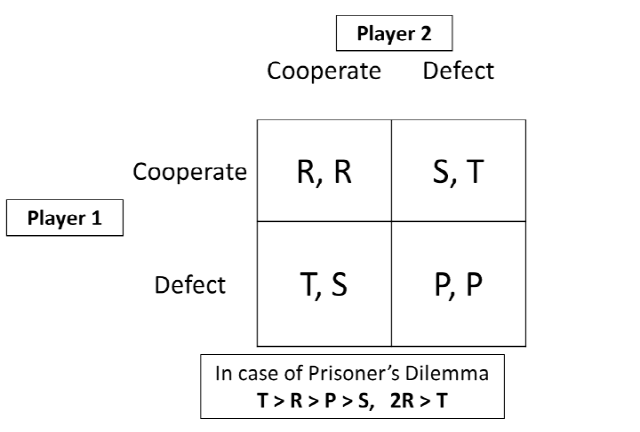
\includegraphics[scale=0.75]{../../other/pd_payoff_matrix.png}
    \caption{Payoff Matrix of Prisoner's Dilemma}
    \label{fig:paymatrix}
\end{figure}

\newpage
As it described in the above, mutual cooperation gives reward payoff $R$ both players, and one defection between two players gives temptation payoff $T$ for defector which is larger than $R$ so that it induces the player to defect when the opponent cooperates and sucker's payoff $S$ for sucker. In case of mutual defection, they will get punishment $P$ payoff whish is larger than $S$ so that it also induces the player to defect when the opponent defect. In sum, everybody is expected to defect, called the \textit{"tragedy of the commons"} (Hardin, 1968).


\subsection{Spatial Game with Strategies}

We simply model social interactions on the $L \times L$ 2-dimensional spatial grid [1]. There are $N$ individuals occupying grid sites with the ratio $\rho$, and they interact with $m$ direct neighbors (von Neumann neighborhoods). The overall payoff $P$ of player $i$ at iteration $t$ is the sum of each payoffs resulting from binary interactions with all von Neumann neighbors [2], and the respective player "imitate" the strategy of best performing neighbor.

In addition, we will extend this game by including both success-driven migration and reputation-based migration. Before the imitation step, a player can move to improve their expected overall payoff to empty site within a quadratic area of $(2M+1) \times (2M+1)$ sites (the Moore neighborhood of size $M$, e.g. the 8 neighboring sites for $M = 1$). A player can also evaluate the surrounding environment and decide whether he leaves or not by comparing his reputation and those of his neighbors [3]. Below equations account for the reputation effect in mobility:

\begin{figure}[!htbp]
	\centering
	
\includegraphics[scale=0.75]{../../other/reputation_eq.png}
    \caption{Reputation Equations}
    \label{fig:reputationeq}
\end{figure}

\section{Implementation}

\section{Simulation Results and Discussion}

\section{Summary and Outlook}

\section{References}

\begin{enumerate}
\item Helbing, D., \& Yu, W. (2009). The outbreak of cooperation among success-driven individuals under noisy conditions. \textit{Proceedings of the National Academy of Sciences, 106}(10), 3680-3685.
\item Helbing, D., Yu, W., \& Rauhut, H. (2011). Self-organization and emergence in social systems: Modeling the coevolution of social environments and cooperative behavior. \textit{The Journal of Mathematical Sociology, 35}(1-3), 177-208.
\item Cong, R., Wu, B., Qiu, Y., \& Wang, L. (2012). Evolution of cooperation driven by reputation-based migration. \textit{PloS one, 7}(5), e35776.
\end{enumerate}









\end{document}  



 
